% Metódy inžinierskej práce

\documentclass[10pt,twocolumn,twoside,slovak,a4paper]{article}

\usepackage[slovak]{babel}
%\usepackage[T1]{fontenc}
\usepackage[T1]{fontenc} % lepšia sadzba písmena Ľ než v T1
\usepackage[utf8]{inputenc}
\usepackage{graphicx}
\usepackage{url} % príkaz \url na formátovanie URL
\usepackage{hyperref} % odkazy v texte budú aktívne (pri niektorých triedach dokumentov spôsobuje posun textu)
\usepackage{todonotes}
\usepackage{cite}
\usepackage{fancyhdr}
\usepackage{wrapfig}
%\usepackage{times}

\pagestyle{fancy}
\fancyhead{}



\title{Je odporúčací systém Netflix-u problém ?\thanks{Semestrálny projekt v predmete Metódy inžinierskej práce, ak. rok 2024/2025, vedenie: Mgr. Yevheniia Kataieva, PhD.}}

\author{Adam Glogovský\\[2pt]
	{\small Slovenská technická univerzita v Bratislave}\\
	{\small Fakulta informatiky a informačných technológií}\\
	{\small \texttt{xglogovsky@stuba.sk}}}

\date{\small 5. október 2024} 



\begin{document}

\maketitle

\section*{Abstract}
Touto prácou by som chcel poukázať na to, ako Netflix ako firma spracúva užívateľské informácie a či je to správne. Na začiatku tejto práce objasním problematiku všeobecných odporúčacích systémov. Potom ukážem kde Netflix posiela užívateľské informácie. Ako ich spracúva a ako podľa nich dokáže nám užívateľom spríjemniť fungovanie na platforme. Ak nám to zvyšuje zážitok z používania tejto platformy, čo to teda tú platformu stojí a či je to vo výsledku pre danú platformu efektívne a finančne prospešné. Taktiež sa pokúsim čo naviac priblížiť samotné spracovanie týchto údajov a poukážem na to, či je správne daným spôsobom spracúvať tieto informácie.\cite{amatriain2015recommender} Dôležítý taktiež pre platformu je, algoritmus akým spracúvajú dané informácie a samotná infraštruktúra v ktorej to celé funguje. Samozrejme touto prácou chcem zistiť, či kvôli tomuto alogritmu a spôsobu spracovania informácií, Netflix neubližuje menej populárnemu alebo menej ''mainstream'' obsahu, ktorý je teda ešte o to menej ukazovaný užívateľom. A tiež poukážem na to, či je tento menej populárny obsah iba nefavoritizovaný a posúvaný nižšie v hľadaní, alebo je kompletne zahaľovaný určitým užívateľom. Na konci tejto práce teda budete vedieť ako Netflix spracúva informácie, či je správne spracovávať užívateľské informácie týmto spôsobom, či je to profitabilné pre Netflix a taktiež, či to prospieva užívateľom tejto platformy.\todo{204 slov}

%\begin{wrapfigure}{r}{0.5\textwidth}
\begin{figure*}
	\centering
	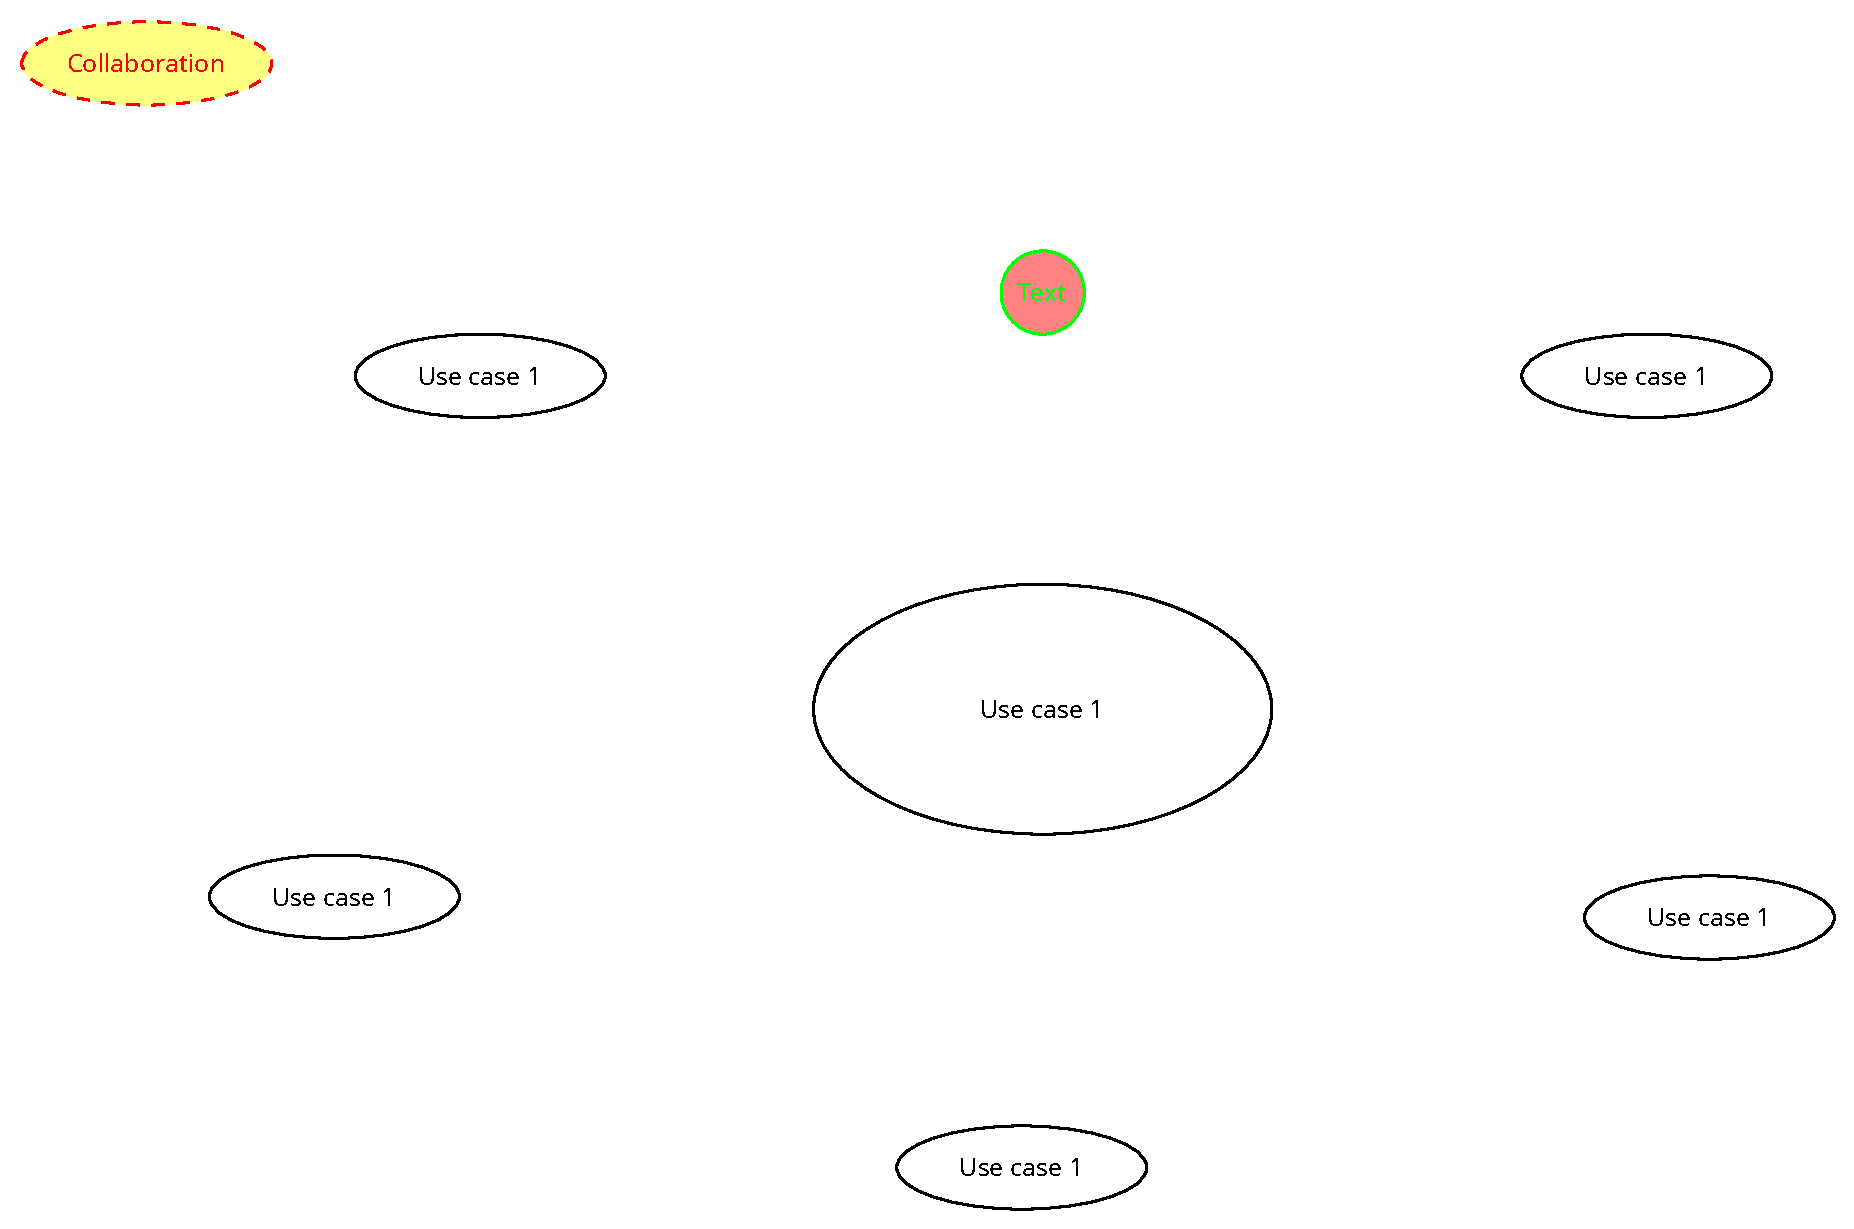
\includegraphics[scale=0.2]{diagram.pdf}
	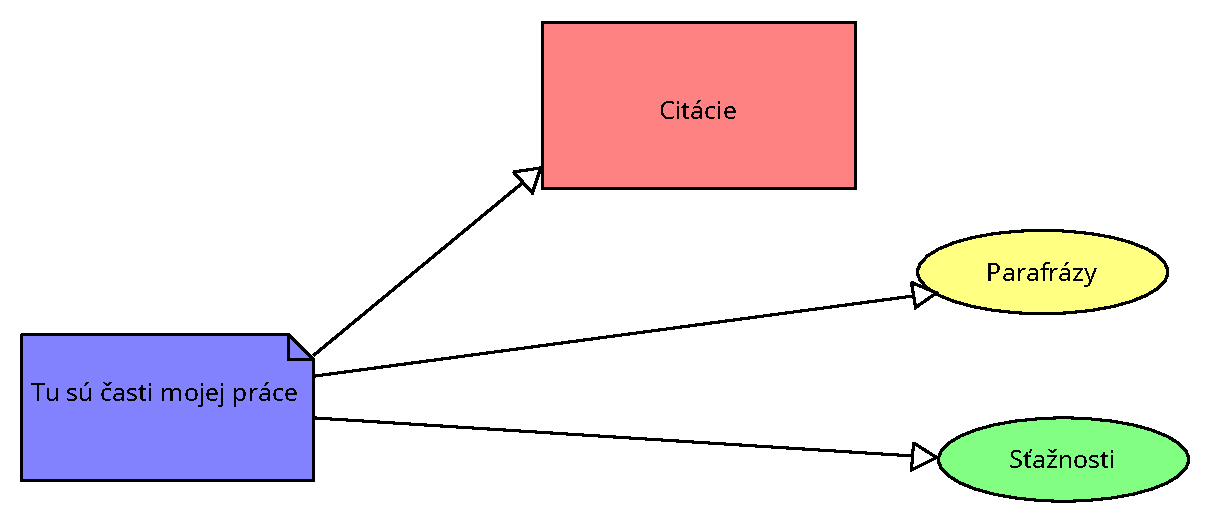
\includegraphics[scale=0.4]{diagram horizontal.pdf}
\end{figure*}
%\end{wrapfigure}





\newpage

%\acknowledgement{Ak niekomu chcete poďakovať\ldots}


% týmto sa generuje zoznam literatúry z obsahu súboru literatura.bib podľa toho, na čo sa v článku odkazujete
\begin{figure}
	\bibliography{literatura}
	\bibliographystyle{abbrv} % prípadne alpha, abbrv alebo hociktorý iný
\end{figure}

\end{document}
